\chapter{Tools}

This chapter provides a overview of the various tools that are
provided as part of the Ames Stereo Pipeline, and a summary of their
command line options.

%--------------------------------------------------------------------------
%                                ASP DEBUGGING
%--------------------------------------------------------------------------

\section{stereo}
\label{stereo}

The \texttt{stereo} program is the primary tool of the Ames
Stereo Pipeline.  It takes a stereo pair of images that overlap and
creates an output point cloud image that can be processed into a 3D
model or DEM using the \texttt{point2mesh} or \texttt{point2dem}
programs, respectively.

\medskip

Usage:\\
\hspace*{2em}\texttt{ISIS 3> stereo [options] \textit{Left\_input\_image Right\_input\_image output\_file\_prefix}}

\medskip

This tool is is primarily designed to process USGS ISIS \texttt{.cub}
files and Digital Globe data. However, Stereo Pipeline
does have the capability to process other types of stereo image pairs
(e.g., image files with a CAHVOR camera model from the NASA MER
rovers).  If you would like to experiment with these features, please
contact us for more information.

The \texttt{\textit{output\_file\_prefix}} is prepended to all
output data files.  For example, setting \texttt{\textit{output\_file\_prefix}}
to `\texttt{out}' will yield files with names like \texttt{out-L.tif}
and \texttt{out-PC.tif}.  To keep the Stereo Pipeline results organized
in sub-directories, we recommend using an output prefix like
`\texttt{results-10-12-09/out}' for \texttt{\textit{output\_file\_prefix}}.  The
\texttt{stereo} program will create a directory called
\texttt{results-10-12-09/out} and place files named \texttt{out-L.tif},
\texttt{out-PC.tif}, etc. in that directory.

\begin{longtable}{|l|p{7.5cm}|}
\caption{Command-line options for stereo}
\label{tbl:stereo}
\endfirsthead
\endhead
\endfoot
\endlastfoot
\hline
Option & Description \\ \hline \hline
\texttt{-\/-help|-h} & Display the help message\\ \hline
\texttt{-\/-threads \textit{integer(=0)}} & Set the number threads to use. 0 means use default defined in the program or in the .vwrc file\\ \hline
\texttt{-\/-session-type|-t pinhole|isis|dg|rpc} & Select the stereo session type to use for processing. Usually the program can select this automatically by the file extension.\\ \hline
\texttt{-\/-stereo-file|-s \textit{filename(=./stereo.default)}} & Define the stereo.default file to use\\ \hline
\texttt{-\/-left-image-crop-win \textit{xoff yoff xsize ysize}}  & Do stereo in a subregion of the left image [default: use the entire image].\\ \hline
\texttt{-\/-entry-point|-e 1|2|3|4} & Stereo Pipeline entry point \\ \hline
\end{longtable}

More information about the stereo.default configuration file can be
found in Appendix \ref{ch:stereodefault} on page
\pageref{ch:stereodefault}.  Similarly, \texttt{stereo} creates a lot
of files, and they are all described in Appendix
\ref{chapter:outputfiles} on page \pageref{chapter:outputfiles}.

\subsection{Entry Points}
\label{entrypoints}

The \texttt{stereo -e \textit{number}} option can be used to restart
a {\tt stereo} job partway through the stereo correlation process.
Restarting can be useful when debugging while iterating on {\tt
stereo.default} settings.

Stage 0 (Preprocessing) normalizes the two images and aligns them
by locating interest points and matching them in both images. The
program is designed to reject outlying interest points.  This stage
writes out the pre-aligned images and the image masks.

Stage 1 (Disparity Map Initialization) performs pyramid correlation and builds a rough disparity map that is used to seed the sub-pixel refinement phase.

Stage 2 (Sub-pixel Refinement) performs sub-pixel correlation that
refines the disparity map.

Stage 3 (Outlier Rejection and Hole Filling) performs filtering of the
disparity map and (optionally) fills in holes using an inpainting
algorithm.  This phase also creates a ``good pixel'' map.

Stage 4 (Triangulation) generates a 3D point cloud from the disparity
map.

\subsection{Decomposition of Stereo}
\label{stereo_dec}

The \texttt{stereo}
executable is a python script that makes calls to separate
C++ executables for each entry point.

Stage 0 (Preprocessing) calls \texttt{stereo\_pprc}. Multi-threaded.

Stage 1 (Disparity Map Initialization) calls
\texttt{stereo\_corr}. Multi-threaded.

Stage 2 (Sub-pixel Refinement) class \texttt{stereo\_rfne}. Multi-threaded.

Stage 3 (Outlier Rejection and Hole Filling) calls
\texttt{stereo\_fltr}. Multi-threaded.

Stage 4 (Triangulation) calls \texttt{stereo\_tri}. Multi-threaded,
except for ISIS input data.

All of the sub-programs have the same interface as
\texttt{stereo}. Users processing a large number of stereo pairs on a
cluster may find it advantageous to call these executables in their own
manner. An example would be to run stages 0-3 in order for each stereo
pair. Then run several sessions of \texttt{stereo\_tri} since it is
single-threaded for ISIS.

It is important to note that each of the C++ stereo executables invoked
by \texttt{stereo} have their own command-line options. Those options
can be passed to \texttt{stereo} which will in turn pass them to the
appropriate executable. By invoking each executable with no options, it
will display the list of options it accepts. As explained in more detail
in section \ref{perform-stereo}, each such option has the same syntax as
used in \texttt{stereo.default}, while being prepended by a double hyphen
(\texttt{-\/-}).  A command line option takes precedence over the same
option specified in \texttt{stereo.default}.

\section{parallel\_stereo}
\label{parallel}

The \texttt{parallel\_stereo} program is a modification of \texttt{stereo}
designed to distribute the stereo processing over multiple computing
nodes.

It uses GNU Parallel to manage the jobs, which needs to be installed
on your system.

Note that, when invoking this tool, only stages 1, 2, and 4 of
stereo (section \ref{stereo_dec}) are spread over multiple machines,
with stages 0 and 3 still being done on the current computing node, as
they require global knowledge of the data. In addition, not all stages
of stereo benefit equally from parallelization, most likely to gain
are stages 1 and 2 (correlation and refinement), which are the most
computationally expensive.

For these reasons, while \texttt{parallel\_stereo} can be called to do
all stages of stereo generation from start to finish in one command, it
may be more resource-efficient to invoke it using a single node for
stages 0 and 3, many nodes for stages 1 and 2, and just a handful of
nodes for stage 4 (triangulation). The example below explains how to do
that.

\texttt{parallel\_stereo} accepts the following options (any additional
options given to it will be passed to the stereo executables
for each stage).

\begin{longtable}{|l|p{7.5cm}|}
\caption{Command-line options for parallel\_stereo}
\label{tbl:parallelstereo}
\endfirsthead
\endhead
\endfoot
\endlastfoot
\hline
Options & Description \\ \hline \hline
\texttt{-\/-help|-h} & Display the help message.\\ \hline
\texttt{-\/-nodes-list \textit{filename} } & The list of computing nodes,
one per line. If not provided, run on the local machine. \\ \hline
\texttt{-\/-processes \textit{integer(=4)}} & The number of processes to
use per node. \\ \hline
\texttt{-\/-threads-multiprocess \textit{integer(=2)}} & The number of threads to use per process.\\ \hline
\texttt{-\/-threads-singleprocess \textit{integer(=1)}} & The number of threads to use when running a single process (for pre-processing and filtering).\\ \hline
\texttt{-\/-entry-point|-e integer(=0 to 5)} & Stereo Pipeline entry
point (start at this stage). \\ \hline
\texttt{-\/-stop-point|-e integer(=1 to 6)} & Stereo Pipeline stop point
(stop at the stage {\it right before} this value). \\ \hline
\texttt{-\/-job-size-w \textit{integer(=2048)}} & Pixel width of input
image tile for a single process. \\ \hline
\texttt{-\/-job-size-h \textit{integer(=2048)}} & Pixel height of input
image tile for a single process. \\ \hline
\end{longtable}

As an example, assume that we would like to launch the refinement and
filtering steps only (stages 2 and 3). We will distribute the
refinement over a number of nodes, using 4 processes on each node, with
each process creating 16 threads. For the filtering stage, which is done
in one process on one machine, we want to use 32 threads. The
appropriate command is then:

\begin{verbatim}
parallel_stereo --nodes-list machines.txt --processes 4 --threads-multiprocess 16 \
 --threads-singleprocess 32 --entry-point 2 --stop-point 4 <other stereo options>
\end{verbatim}

Note that, if \texttt{parallel\_stereo} is launched as a supercomputer
job, the path to the file containing the list of nodes may exist as an environmental
variable. For example, on NASA's Pleiades Supercomputer, which uses the
Portable Batch System (PBS), the list of computing nodes currently
available can be retrieved as \$PBS\_NODEFILE.

\section{disparitydebug}
\label{disparitydebug}

The \texttt{disparitydebug} program produces output images for
debugging disparity images created from \verb#stereo#. The {\tt
stereo} tool produces several different versions of the disparity
map; the most important ending with extensions \verb#*-D.tif# and
\verb#*-F.tif#. (see Appendix \ref{chapter:outputfiles} for more
information.)  These raw disparity map files can be useful for
debugging because they contain raw disparity values as measured by
the correlator; however they cannot be directly visualized or opened
in a conventional image browser.  The \verb#disparitydebug# tool
converts a single disparity map file into two normalized TIFF image
files (\verb#*-H.tif# and \verb#*-V.tif#, containing the horizontal
and vertical, or line and sample, components of disparity, respectively)
that can be viewed using any image display program.

The {\tt disparitydebug} program will also print out the range of
disparity values in a disparity map, that can serve as useful summary
statistics when tuning the search range settings in the
{\tt stereo.default} file.

\begin{longtable}{|l|p{10cm}|}
\caption{Command-line options for disparitydebug}
\label{tbl:disparitydebug}
\endfirsthead
\endhead
\endfoot
\endlastfoot
\hline
Options & Description \\ \hline \hline
\texttt{-\/-help|-h} & Display the help message\\ \hline
\texttt{-\/-input-file \textit{filename}} & Explicitly specify the input file \\ \hline
\texttt{-\/-output-prefix|-o \textit{filename}} & Specify the output file prefix \\ \hline
\texttt{-\/-output-filetype|-t \textit{type(=tif)}} & Specify the outfile type \\ \hline
\texttt{-\/-float-pixels} & Save the resulting debug images as 32 bit floating point files (if supported by the selected file type) \\ \hline
\end{longtable}

%--------------------------------------------------------------------------
%                           VISUALIZATION TOOLS
%--------------------------------------------------------------------------

\section{point2dem}
\label{point2dem}

The \texttt{point2dem} program produces a GeoTIFF terrain model or/and
an orthographic image from a point cloud image produced by the {\tt
  stereo} command.

Example:\\
\hspace*{2em}\texttt{point2dem \textit{output-prefix}-PC.tif -o stereo/filename -r moon $\backslash$} \\
\hspace*{4em}\texttt{-\/-nodata-value -10000 -n}

This produces a digital elevation model that has been referenced to
the lunar spheroid of 1737.4~km.  Pixels with no data will be set to a
value of -10000, and the resulting \ac{DEM} will be saved in a simple
cylindrical map-projection.  The resulting \ac{DEM} is stored by default as
a one channel, 32-bit floating point GeoTIFF file.

The {\tt -n} option creates an 8-bit, normalized version of the DEM
that can be easily loaded into a standard image viewing application
for debugging.

Another example: \\
\hspace*{2em}\texttt{point2dem \textit{output-prefix}-PC.tif -o stereo/filename -r moon $\backslash$} \\
\hspace*{4em}\texttt{-\/-orthoimage \textit{output-prefix}-L.tif}

This command takes the left input image and orthographically projects
it onto the 3D terrain produced by the Stereo Pipeline.  The resulting
{\tt *-DRG.tif} file will be saved as an 8-bit GeoTIFF image in a
simple cylindrical map-projection.

\subsection{Comparing with MOLA Data}

When comparing the output of \texttt{point2dem} to laser altimeter
data, like MOLA, it is important to understand the different kinds
of data that are being discussed.  By default, \texttt{point2dem}
returns planetary radius values in meters.  These are often large
numbers that are difficult to deal with.  If you use the \texttt{-r
mars} option, the output terrain model will be in meters of elevation
with reference to the IAU reference spheroid for Mars: 3,396,190~m.
So if a post would have a radius value of 3,396,195~m, in the model
returned with the \texttt{-r mars} option, that pixel would just be 5~m.

You may want to compare the output to MOLA data.  MOLA data is
released in three `flavors,' namely: Topography, Radius, and Areoid.
The MOLA Topography data product that most people use is just the MOLA Radius
product with the MOLA Areoid product subtracted.  Additionally, it is
important to note that all of these data products have a reference
value subtracted from them.  The MOLA reference value is NOT the
IAU reference value, but 3,396,000~m.

In order to compare with the MOLA data, you can do one of two
different things.  You could operate purely in radius space, and
have \texttt{point2dem} create radius values that are directly
comparable to the MOLA Radius data.  You can do this by having
\texttt{point2dem} subtract the MOLA reference value by setting
\texttt{-\/-semi-major-axis 3396000} and \texttt{-\/-semi-minor-axis
3396000}.

To get values that are directly comparable to MOLA Topography data,
you'll need to run \texttt{point2dem} with the option \texttt{-r mars},
then run the ASP tool \texttt{dem\_geoid} (section \ref{demgeoid}). This
program will convert the DEM height values from being relative to the IAU
reference spheroid to being relative to the MOLA Areoid.

\subsection{Post Spacing}

Recall that \texttt{stereo} creates a point cloud file as its output
that you need to use \texttt{point2dem} on to create a GeoTIFF that
you can use in other tools.  The point cloud file is the result of
taking the image-to-image matches (which were created from the
kernel sizes you specified, and the subpixel versions of the same,
if used) and projecting them out into space from the cameras, and
arriving at a point in real world coordinates.  Since \texttt{stereo} does
this for every pixel in the input images, the \emph{default} value that
\texttt{point2dem} uses (if you don't specify anything explicitly) is: the
input image scale, because there's an `answer' in the point cloud
file for each pixel in the original image.

However, as you may suspect, this is probably not the best value to
use, because there really isn't that much `information' in the data.
The true `resolution' of the output model is dependent on a whole
bunch of things (like the kernel sizes you choose to use) but also can
vary from place to place in the image depending on the texture.

The general `rule of thumb' is to produce a terrain model that has a
post spacing of about 3x the input image ground scale.  This is based
on the fact that it is nearly impossible to uniquely identify a single
pixel correspondence between two images, but a 3x3 patch of pixels
provides improved matching reliability.  As you go to numerically
larger post-spacings on output, you're averaging more point data (that
is probably spatially correlated anyway) together.

So you can either use the \texttt{-\/-dem-spacing} argument to
\texttt{point2dem} to do that directly, or feel free to use your
favorite averaging algorithm to reduce the \texttt{point2dem}-created
model down to the scale you want.

If you attempt to derive science results from an ASP-produced terrain model
with the default DEM spacing, expect serious questions from reviewers.


\begin{longtable}{|p{8cm}|p{9cm}|}
\caption{Command-line options for point2dem}
\label{tbl:point2dem}
\endfirsthead
\endhead
\endfoot
\endlastfoot
\hline
Options & Description \\ \hline \hline
\texttt{-\/-nodata-value \textit{float(=min-z)}} & Explicitly set the default missing pixel value. By default, the minimum z value in the model is used. \\ \hline
\texttt{-\/-use-alpha} & Create images that have an alpha channel \\ \hline
\texttt{-\/-normalized|-n} & Also write a normalized version of the \ac{DEM} (for debugging) \\ \hline
\texttt{-\/-orthoimage \textit{texture-file}} & Write an orthoimage based on the texture file given as an argument to this command line option \\ \hline
\texttt{-\/-errorimage} & Write an additional image whose values represent the triangulation error in meters \\ \hline
\texttt{-\/-fsaa  \textit{float(=3)}} & Oversampling amount to perform antialiasing. \\ \hline
\texttt{-\/-output-prefix|-o \textit{output-prefix}} & Specify the output prefix \\ \hline
\texttt{-\/-output-filetype|-t \textit{type(=tif)}} & Specify the output file type \\ \hline
\hline
\texttt{-\/-x-offset \textit{float(=0)}} & Add a horizontal offset to the \ac{DEM} \\ \hline
\texttt{-\/-y-offset \textit{float(=0)}} & Add a horizontal offset to the \ac{DEM} \\ \hline
\texttt{-\/-z-offset \textit{float(=0)}} & Add a vertical offset to the \ac{DEM} \\ \hline
\texttt{-\/-rotation-order \textit{order(=xyz)}} & Set the order of an Euler angle rotation applied to the 3D points prior to \ac{DEM} rasterization \\ \hline
\texttt{-\/-phi-rotation \textit{float(=0)}} & Set a rotation angle phi \\ \hline
\texttt{-\/-omega-rotation \textit{float(=0)}} & Set a rotation angle omega \\ \hline
\texttt{-\/-kappa-rotation \textit{float(=0)}} & Set a rotation angle kappa \\ \hline
\hline
\texttt{-\/-t\_srs \textit{string}} & Target spatial reference set. This mimics the GDAL option used on their tools. \\ \hline
\texttt{-\/-reference-spheroid|-r moon|mars} & Set a reference surface to a hard coded value. This will override manually set datum information. \\ \hline
\texttt{-\/-semi-major-axis \textit{float(=0)}} & Set the dimensions of the datum in meters\\ \hline
\texttt{-\/-semi-minor-axis \textit{float(=0)}} & Set the dimensions of the datum in meters\\ \hline
\texttt{-\/-sinusoidal} & Save using a sinusoidal projection \\ \hline
\texttt{-\/-mercator} & Save using a Mercator projection \\ \hline
\texttt{-\/-transverse-mercator} & Save using transverse Mercator projection \\ \hline
\texttt{-\/-orthographic} & Save using an orthographic projection \\ \hline
\texttt{-\/-stereographic} & Save using a stereographic projection \\ \hline
\texttt{-\/-lambert-azimuthal} & Save using a Lambert azimuthal projection \\ \hline
\texttt{-\/-utm \textit{zone}} & Save using a UTM projection with the given zone \\ \hline
\texttt{-\/-proj-lat \textit{float}} & The center of projection latitude (if applicable) \\ \hline
\texttt{-\/-proj-lon \textit{float}} & The center of projection longitude (if applicable) \\ \hline
\texttt{-\/-proj-scale \textit{float}} & The projection scale (if applicable) \\ \hline
\texttt{-\/-dem-spacing|-s \textit{float(=0)}} & Set the \ac{DEM} post size (if this value is 0, the post spacing size is computed for you) \\ \hline
\texttt{-\/-rounding-error \textit{float(=$1/2^{10}$=$0.0009765625$)}} & How much to round the output DEM and errors, in meters (more rounding means less precision but potentially smaller size on disk). The inverse of a power of 2 is suggested. \\ \hline
\texttt{-\/-threads \textit{int(=0)}} & Select the number of processors (threads) to use.\\ \hline
\texttt{-\/-no-bigtiff} & Tell GDAL to not create bigtiffs.\\ \hline
\texttt{-\/-tif-compress None|LZW|Deflate|Packbits} & TIFF compression method.\\ \hline
\texttt{-\/-cache-dir \textit{directory(=/tmp)}} & Folder for temporary files. Normally this need not be changed.\\ \hline
\hline
\texttt{-\/-help|-h} & Display the help message \\ \hline
\end{longtable}

\section{point2mesh}
\label{point2mesh}

Produces a mesh surface that can be visualized in {\tt osgviewer},
which is a standard 3D viewing application that is part of the open
source OpenSceneGraph package.  \footnote{The full OpenSceneGraph package
is not bundled with the Stereo Pipeline, but the \texttt{osgviewer} program
is.  You can download and install this package separately from
\url{http://www.openscenegraph.org/}.}

Unlike \acp{DEM}, the 3D mesh is not meant to be used as a finished
scientific product.  Rather, it can be used for fast visualization
to create a 3D view of the generated terrain.

The \texttt{point2mesh} program requires a point cloud file and an
optional texture file (\texttt{\textit{output-prefix}-PC.tif} and
normally \texttt{\textit{output-prefix}-L.tif}). When a texture
file is not provided, a 1D texture is applied in the local Z direction
that produces a rough rendition of a contour map.  In either case,
\texttt{point2mesh} will produce a \texttt{\textit{output-prefix}.ive}
file that contains the 3D model in OpenSceneGraph format.

Two options for \texttt{osgviewer} bear pointing out: the \texttt{-l}
flag indicates that synthetic lighting should be activated for the
model, which can make it easier to see fine detail in the model by
providing some real-time, interactive hillshading.  The \verb#-s#
flag sets the sub-sampling rate, and dictates the degree to which
the 3D model should be simplified.  For 3D reconstructions, this
can be essential for producing a model that can fit in memory.  The
default value is 10, meaning every 10th point is used in the X and
Y directions. In other words that mean only $1/10^2$ of the points
are being used to create the model. Adjust this sampling rate
according to how much detail is desired, but remember that large
models will impact the frame rate of the 3D viewer and affect
performance.

Example:\\
\hspace*{2em}\texttt{point2mesh -l -s 2 \textit{output-prefix}-PC.tif \textit{output-prefix}-L.tif}

To view the resulting \texttt{\textit{output-prefix}.ive} file use
\texttt{osgviewer}.

\hspace*{2em}Fullscreen:\\
\hspace*{2em}\texttt{> osgviewer \textit{output-prefix}.ive}

\hspace*{2em}or Windowed:\\
\hspace*{2em}\texttt{> osgviewer \textit{output-prefix}.ive -\/-window 50 50 1000 1000}

Inside \texttt{osgviewer}, the keys L, T, and W can be used to toggle on
and off lighting, texture, and wireframe modes.  The left, middle, and
right mouse buttons control rotation, panning, and zooming of the
model.

\begin{longtable}{|l|p{10cm}|}
\caption{Command-line options for point2mesh}
\label{tbl:point2mesh}
\endfirsthead
\endhead
\endfoot
\endlastfoot
\hline
Options & Description \\ \hline \hline
\texttt{-\/-help|-h} & Display the help message\\ \hline
\texttt{-\/-simplify-mesh \textit{float}} & Run OSG Simplifier on mesh, 1.0 = 100\% \\ \hline
\texttt{-\/-smooth-mesh} & Run OSG Smoother on mesh \\ \hline
\texttt{-\/-use-delaunay} & Uses the delaunay triangulator to create a surface from the point cloud. This is not recommended for point clouds with noise issues. \\ \hline
\texttt{-\/-step|-s \textit{integer(=10)}} & Sampling step size for mesher. \\ \hline
\texttt{-\/-input-file \textit{pointcloud-file}} & Explicitly specify the input file \\ \hline
\texttt{-\/-texture-file \textit{texture-file}} & Explicitly specify the texture file \\ \hline
\texttt{-\/-output-prefix|-o \textit{output-prefix}} & Specify the output prefix \\ \hline
\texttt{-\/-output-filetype|-t \textit{type(=ive)}} & Specify the output file type \\ \hline
\texttt{-\/-enable-lighting|-l} & Enables shades and light on the mesh \\ \hline
\texttt{-\/-center} & Center the model around the origin. Use this option if you are experiencing numerical precision issues. \\ \hline
\texttt{-\/-rotation-order \textit{order(=xyz)}} & Set the order of an euler angle rotation applied to the 3D points prior to DEM rasterization \\ \hline
\texttt{-\/-phi-rotation \textit{float(=0)}} & Set a rotation angle phi \\ \hline
\texttt{-\/-omega-rotation \textit{float(=0)}} & Set a rotation angle omega \\ \hline
\texttt{-\/-kappa-rotation \textit{float(=0)}} & Set a rotation angle kappa \\ \hline
\end{longtable}

\section{mapproject}
\label{mapproject}

The tool \texttt{mapproject} is used to map-project a camera image onto
a DEM. The obtained images can be used, for example, to visualize how
camera images would look when projected onto the ground obtained by
doing stereo of these images (ideally, if there were no correlation or
triangulation error, the images would project perfectly). The tool can
also be used to compute stereo from the obtained map-projected images;
this functionality is currently supported only with RPC models (section
\ref{mapproj}).

\texttt{mapproject} supersedes the older
\texttt{orthoproject} tool, which could map-project only with ISIS and
pinhole camera models (the latter program is still being kept for a few
releases for backward compatibility). We ported all features of
\texttt{orthoproject} except for projecting of vector imagery (for
example, RGB pixel data).

\texttt{mapproject} is single-threaded for ISIS cameras, this is due to
the limitations of ISIS. At some point this tool will be able to
distribute itself using multiple processes to work around this limitation.


Example:
\begin{verbatim}
mapproject -t isis DEM.tif image.cub camera.isis_adjust \
         output-IMG.tif --ppd 256
\end{verbatim}

\begin{longtable}{|l|p{10cm}|}
\caption{Command-line options for mapproject}
\label{tbl:mapproject}
\endfirsthead
\endhead
\endfoot
\endlastfoot
\hline
Options & Description \\ \hline \hline
\texttt{-\/-nodata-value \textit{double(=-32768)}} & No-data value to use unless specified in the input image. \\ \hline
\texttt{-\/-t\_srs} & Target spatial reference set. This mimics the GDAL
option. If not provided use the one from the DEM. \\ \hline
\texttt{-\/-tr \textit{float}} & Set the output file resolution in target
  georeferenced units per pixel. \\ \hline
\texttt{-\/-mpp \textit{float}} & Set the output file resolution in meters per
pixel. \\ \hline
\texttt{-\/-ppd \textit{float}} & Set the output file resolution in pixels per
degree. \\ \hline
\texttt{-\/-session-type|-t pinhole|isis|dg|rpc} & Select the stereo
session type to use for processing. Usually the program can select this
automatically by the file extension except for DG and RPC.\\ \hline
\texttt{-\/-t\_projwin \textit{xmin ymin xmax ymax}} & Selects a subwindow from the source image for copying, with the corners given in georeferenced coordinates. Max is exclusive. \\ \hline
\texttt{-\/-threads \textit{int(=0)}} & Select the number of processors (threads) to use.\\ \hline
\texttt{-\/-no-bigtiff} & Tell GDAL to not create bigtiffs.\\ \hline
\texttt{-\/-tif-compress None|LZW|Deflate|Packbits} & TIFF compression method.\\ \hline
\texttt{-\/-cache-dir \textit{directory(=/tmp)}} & Folder for temporary files. Normally this need not be changed.\\ \hline
\texttt{-\/-help|-h} & Display the help message\\ \hline
\end{longtable}

\clearpage

\section{orbitviz}
\label{orbitviz}

Produces a Google Earth \ac{KML} file useful for visualizing camera
position. The input for this tool is one or more \texttt{*.cub} files.

\begin{figure}[!b]
  \begin{center}
  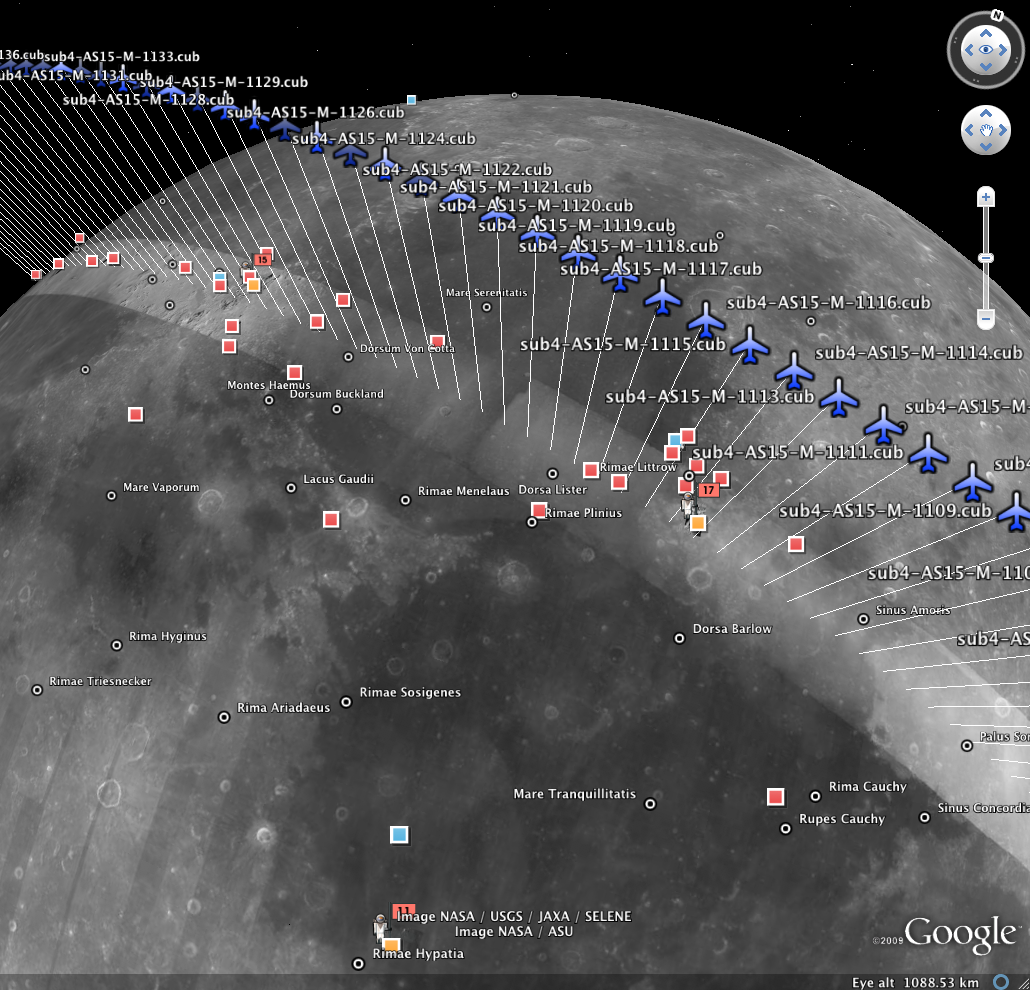
\includegraphics[width=6in]{images/orbitviz_ge_result.png}
  \end{center}
  \caption{ Example of a \ac{KML} visualization produced with {\tt
      orbitviz} depicting camera locations for the Apollo 15 Metric
    Camera during orbit 33 of the Apollo command module.}
  \label{fig:orbitviz_example}
\end{figure}

\begin{longtable}{|l|p{10cm}|}
\caption{Command-line options for orbitviz}
\label{tbl:orbitviz}
\endfirsthead
\endhead
\endfoot
\endlastfoot
\hline
Options & Description \\ \hline \hline
\texttt{-\/-help|-h} & Display the help message\\ \hline
\texttt{-\/-output|-o \textit{filename(=orbit.kml)}} & Specifies the output file name \\ \hline
\texttt{-\/-scale|-s \textit{float(=1)}} & Scale the size of the coordinate axes by this amount. Ex: To scale axis sizes up to earth size, use 3.66 \\ \hline
\texttt{-\/-use\_path\_to\_dae\_model|-u \textit{fullpath}} & Use this dae model to represent camera location. \emph{Google Sketch up can create these.} \\ \hline
\end{longtable}

\clearpage

\section{cam2map4stereo.py}
\label{cam2map4stereo}

This program takes similar arguments as the ISIS3 \texttt{cam2map} program,
but takes two input images.  With no arguments, the program determines
the minimum overlap of the two images, and the worst common resolution,
and then map-projects the two images to this identical area and resolution.

The detailed reasons for doing this, and a manual step-by-step walkthrough of
what \texttt{cam2map4stereo.py} does is provided in the disucssion on aligning images on page \pageref{sec:AligningImages}.

The \texttt{cam2map4stereo.py} is also useful for selecting a subsection and/or reduced resolution portion of the full image.  You can inspect a raw camera geometry image in qview after you have run \texttt{spiceinit} on it, select the latitude and longitude ranges, and then use \texttt{cam2map4stereo.py}'s \texttt{-\/-lat}, \texttt{-\/-lon}, and optionally \texttt{-\/-resolution} options to pick out just the part you want.

Use the \texttt{-\/-dry-run} option the first few times to get an idea of what \texttt{cam2map4stereo.py} does for you.

\begin{longtable}{|l|p{10cm}|}
\caption{Command-line options for cam2map4stereo.py}
\label{tbl:bundlevis}
\endfirsthead
\endhead
\endfoot
\endlastfoot
\hline
Options & Description \\ \hline \hline
\texttt{-\/-help|-h} & Display the help message. \\ \hline
\texttt{-\/-manual} & Read the manual. \\ \hline
\texttt{-\/-map=\textit{MAP}|-m \textit{MAP}} & The mapfile to use for \texttt{cam2map}. \\ \hline
\texttt{-\/-pixres=\textit{PIXRES}|-p \textit{PIXRES}} & The pixel resolution mode to use for \texttt{cam2map}. \\ \hline
\texttt{-\/-resolution=\textit{RESOLUTION}|-r \textit{RESOLUTION}} & Resolution of the final map for \texttt{cam2map}. \\ \hline
\texttt{-\/-interp=\textit{INTERP}|-i \textit{INTERP}} & Pixel interpolation scheme for \texttt{cam2map}. \\ \hline
\texttt{-\/-lat=\textit{LAT}|-a \textit{LAT}} & Latitude range for \texttt{cam2map}, where \texttt{LAT} is of the form \textit{min:max}.  So to specify a latitude range between -5 and 10 degrees, it would look like \texttt{-\/-lat=-5:10}. \\ \hline
\texttt{-\/-lon=\textit{LON}|-o \textit{LON}} & Longitude range for \texttt{cam2map}, where \texttt{LON} is of the form \textit{min:max}.  So to specify a longitude range between 45 and 47 degrees, it would look like \texttt{-\/-lon=40:47}. \\ \hline
\texttt{-\/-dry-run|-n} & Make calculations, and print the \texttt{cam2map} command that would be executed, but don't actually run it.\\ \hline
\texttt{-\/-suffix|-s} & Suffix that gets inserted in the output file names, defaults to `map'.\\ \hline
\end{longtable}

\clearpage

\section{dem\_geoid}
\label{demgeoid}

This tool takes as input a DEM whose height values are relative to the
datum ellipsoid, and adjusts those values to be relative to the
equipotential surface of the planet (geoid on Earth, and areoid on
Mars). The program can also apply the reverse of this adjustment. The
adjustment simply subtracts from the DEM height the geoid height
(correcting, if need be, for differences in dimensions between the DEM
and geoid datum ellipsoids).

Two geoids and one areoid are supported. The Earth geoids are: EGM96, referenced to the WGS84 datum ellipsoid (\url{http://earth-info.nga.mil/GandG/wgs84/gravitymod/egm96/egm96.html})
and NAVD88, referenced to the NAD83 datum ellipsoid (\url{http://www.ngs.noaa.gov/GEOID/GEOID09/}).

The Mars areoid is MOLA MEGDR
(\url{http://geo.pds.nasa.gov/missions/mgs/megdr.html}). When importing
it into ASP, we adjusted the areoid height values to be relative to
the IAU reference spheroid for Mars of radius 3,396,190~m, to be
consistent with the DEM data produced by ASP. The areoid at that source was
relative to the Mars radius of 3,396,000~m.

\begin{longtable}{|l|p{10cm}|}
\caption{Command-line options for dem\_geoid}
\label{tbl:demgeoid}
\endfirsthead
\endhead
\endfoot
\endlastfoot
\hline
Options & Description \\ \hline \hline
\texttt{-\/-help|-h} & Display the help message\\ \hline
\texttt{-\/-nodata-value \textit{integer(=-32768)}} & The value of no-data pixels, unless specified in the DEM \\ \hline
\texttt{-\/-output-prefix|-o \textit{filename}} & Specify the output file prefix \\ \hline
\texttt{-\/-double} & Output using double precision (64 bit) instead of float (32 bit)\\ \hline
\texttt{-\/-reverse-adjustment} & Go from DEM relative to the geoid/areoid to DEM relative to the datum ellipsoid\\ \hline
\end{longtable}

\section{dg\_mosaic}
\label{dgmosaic}

This tool can be used when processing Digital Globe Imagery (section
\ref{sec:digital_globe_imagery}). A Digital Globe satellite may take a
picture, and then split it into several images and corresponding camera XML
files. \texttt{dg\_mosaic} will mosaic these images into a single file,
and create the appropriate combined camera XML file.

Digital Globe camera files contain, in addition to the original camera models, their RPC approximations
(section \ref{rpc}). \texttt{dg\_mosaic} outputs both types of combined models. The combined RPC model can be used to map-project the mosaiced images with the goal of computing stereo from them (section \ref{mapproj}).

The tool needs to be applied twice, for each of the left and right image sets.

\texttt{dg\_mosaic} can also reduce the image resolution while creating the
mosaics (with the camera files modified accordingly).


\begin{longtable}{|l|p{10cm}|}
\caption{Command-line options for dg\_mosaic}
\label{tbl:dgmosaic}
\endfirsthead
\endhead
\endfoot
\endlastfoot
\hline
Options & Description \\ \hline \hline
\texttt{-\/-help|-h} & Display the help message.\\ \hline
\texttt{-\/-gdal-dir \textit{directory}} &
Directory where the GDAL tools are. If not provided, we get them from the environment. \\ \hline
\texttt{-\/-reduce-percent \textit{integer(=100)}} &
Render a reduced resolution image and XML based on this percentage. \\ \hline
\texttt{-\/-skip-rpc-gen \textit{[default: false]}} &
Skip RPC model generation.\\ \hline
\texttt{-\/-rpc-penalty-weight \textit{float(=0.1)}} &
The weight to use to penalize higher order RPC coefficients when generating the combined RPC model. Higher penalty weight results in smaller such coefficients.\\ \hline
\texttt{-\/-output-prefix \textit{string}} & The prefix for the output .tif and .xml files. \\ \hline
\texttt{-\/-input-nodata-value \textit{float}} & Nodata value to use on input; input pixel values less than or equal to this are considered invalid. \\ \hline
\texttt{-\/-output-nodata-value \textit{float}} & Nodata value to use on output. \\ \hline

\texttt{-\/-preview } & Render a small 8 bit png of the input for preview. \\ \hline
\texttt{-\/- \textit{dry-run|-n}} & Make calculations, but just print out the commands. \\ \hline
\end{longtable}

\section{point2las}
\label{point2las}

This tool can be used to convert point clouds generated by ASP to the
public LAS format for interchange of 3-dimensional point cloud data.

\begin{longtable}{|l|p{10cm}|}
\caption{Command-line options for point2las}
\label{tbl:point2las}
\endfirsthead
\endhead
\endfoot
\endlastfoot
\hline
Options & Description \\ \hline \hline
\texttt{-\/-help|-h} & Display the help message.\\ \hline
\texttt{-\/-compressed} &
Compress using laszip. \\ \hline
\texttt{-\/-output-prefix|-o \textit{filename}} & Specify the output file prefix. \\ \hline
\texttt{-\/-threads \textit{integer(=0)}} & Set the number threads to use. 0 means use default defined in the program or in the .vwrc file.\\ \hline
\texttt{-\/-tif-compress None|LZW|Deflate|Packbits} & TIFF compression method.\\ \hline
\texttt{-\/-cache-dir \textit{directory(=/tmp)}} & Folder for temporary files. Normally this need not be changed.\\ \hline
\end{longtable}

\section{pc\_align}
\label{pcalign}

This tool can be used to align two point clouds using Point-to-Plane or
Point-to-Point Iterative Closest Point (ICP). It uses the
\texttt{libpointmatcher} library~\cite{Pomerleau12comp}
(https://github.com/ethz-asl/libpointmatcher).

Several important things need to be kept in mind if \texttt{pc\_align} is to be
used successfully and give accurate results, as described below.

Due to the nature of ICP, the reference (fixed) point cloud should be
denser than the source (movable) point cloud to get the most accurate
results. This is not a serious restriction, as one can perform the
alignment this way and then simply invert the obtained transform if
desired (\texttt{pc\_align} outputs both the direct and inverse
transform, and can output the reference point cloud transformed to match
the source and vice-versa).

In many typical applications, the source and reference point clouds are
already roughly aligned, but the source point cloud may cover a larger
area than the reference. The user should provide to the tool the
expected maximum distance (displacement) source points may move by as
result of alignment, using the option
\texttt{-\/-max-displacement}. This number will help remove source
points too far from the reference point cloud which may not match
successfully and may degrade the accuracy. If in doubt, this value can
be set to something large but still reasonable, as the tool is able to
throw away a certain number of unmatched outliers. At the end of
alignment, \texttt{pc\_align} will display the {\it observed} maximum
displacement, a multiple of which can be used to seed the tool in a
subsequent run.

The user can choose how many points to pick from the reference and
source point clouds to perform the alignment. The amount of memory and
processing time used by \texttt{pc\_align} is directly proportional to
these numbers.

Normally Point-to-Plane ICP is more accurate than Point-to-Point, but
the latter can be good enough if the input point clouds have small
alignment errors, and it uses less storage and memory as well.  The tool
also accepts an option named \texttt{-\/-highest-accuracy}, when it will
compute the normals for Point-to-Plane ICP at all points rather than
about a tenth of them. This option is not necessary most of the time,
but may result in better alignment, at the expense of using more memory
and processing time.

The input point clouds can be in one of several formats: ASP's point
cloud format, DEMs as GeoTiff files, or plain-text CSV files (with .csv
or .txt extension). CSV files are expected to have on each line the
latitude, longitude, and height above the datum (separated by commas or
spaces). The datum itself can be set via the \texttt{-\/-datum} option
(\texttt{pc\_align} attempts to infer the datum from the data if not
provided).  The tool can also read the LOLA RDR PointPerRow format (when
the datum is assumed to be of the Moon).

The transform obtained by \texttt{pc\_align} is output to a file as a
$4\times 4$ matrix, with the upper-left $3\times 3$ submatrix being the
rotation, and the top three elements of the right-most column being the
translation. This matrix can be supplied back to the tool as an initial
guess. The inverse transform is saved to a file as well.

The tool outputs the translation component of this transform, defined
as the vector from the centroid of the original source points to the transformed
centroid. The transform itself, with its origin at the center of the planet,
can result in large movements on the planet surface even for small angles
of rotation, as such both its rotation and translation components may not
be amenable to good interpretation.

The tool outputs to a file the complete list of errors together with
their location, where an error is defined as the distance from a source
point to the closest reference point. It displays the 16th, 50th, and
84th error percentiles, as well as the means of the smallest 25\%, 50\%,
75\%, and 100\% of the errors, all these before and after alignment
transform is applied to the source points.

By default, when \texttt{pc\_align} discards
outliers during the computation of the alignment transform, it keeps
the 75\% of the points with the smallest errors. As such, a way of
judging the effectiveness of the tool is to look at the mean of the
smallest 75\% of the errors before and after alignment.

\medskip

Usage:\\
\hspace*{2em}\texttt{pc\_align -\/-max-displacement arg [other options] <reference cloud> <source cloud>}

\medskip

\begin{longtable}{|p{8cm}|p{9cm}|}
\caption{Command-line options for pc\_align}
\label{tbl:pcalign}
\endfirsthead
\endhead
\endfoot
\endlastfoot
\hline
Options & Description \\ \hline \hline
\texttt{-\/-help|-h} & Display the help message.\\ \hline
\texttt{-\/-threads \textit{integer(=0)}} & Set the number threads to
use. 0 means use the default as set by OpenMP. Only some parts of the algorithm are multi-threaded.\\ \hline
\texttt{-\/-initial-transform \textit{arg}} &
The file containing the rotation + translation transform to be used as an
initial guess. It can come from a previous run of the tool. \\ \hline
\texttt{-\/-num-iterations \textit{default: 1000}} &  Maximum number of iterations. \\ \hline
\texttt{-\/-diff-rotation-error \textit{default: $10^{-8}$}} & Change in rotation amount below which the algorithm will stop, in degrees. \\ \hline
\texttt{-\/-diff-translation-error \textit{default: $10^{-3}$}} & Change in translation amount below which the algorithm will stop, in meters. \\ \hline
\texttt{-\/-max-displacement \textit{arg}} & Maximum expected
displacement of source points as result of alignment, in meters (after
the initial guess transform is applied to the source points). Used
for removing gross outliers in the source (movable) point cloud.\\ \hline
\texttt{-\/-outlier-ratio \textit{default: 0.75}} &  Fraction of source (movable) points considered inliers (after gross outliers further than max-displacement from reference points are removed). \\ \hline
\texttt{-\/-max-num-reference-points \textit{default: $10^8$}} &
Maximum number of (randomly picked) reference points to use. \\ \hline
\texttt{-\/-max-num-source-points \textit{default: $10^5$}} & Maximum number of (randomly picked) source points to use (after discarding gross outliers). \\ \hline
\texttt{-\/-alignment-method \textit{default: point-to-plane}} & The type of iterative closest point
method to use. [point-to-plane, point-to-point]\\ \hline
\texttt{-\/-highest-accuracy} & Compute with highest accuracy for point-to-plane (can be much slower). \\ \hline
\texttt{-\/-datum \textit{}} & Use this datum for CSV files instead of
auto-detecting it. [WGS\_1984, D\_MOON, D\_MARS, etc.] \\ \hline
\texttt{-\/-config-file \textit{file.yaml}} & This is an advanced
option. Read the alignment parameters from a configuration file, in the
format expected by libpointmatcher, over-riding the command-line options.\\ \hline
\texttt{-\/-output-prefix|-o \textit{filename}} & Specify the output file prefix. \\ \hline
\texttt{-\/-compute-translation-only} & Compute the transform from source to reference point cloud as a translation only (no rotation). \\ \hline
\texttt{-\/-save-transformed-source-points} & Apply the obtained transform to the source points so they match the reference points and save them. \\ \hline
\texttt{ -\/-save-inv-transformed-reference-points} & Apply the inverse of the obtained transform to the reference points so they match the source points and save them.
\\ \hline
\end{longtable}




\section{lronac2mosaic.py}
\label{lronac2mosaic}

This tool takes in two LRONAC files (M*LE.IMG and M*RE.IMG) and
produces a single noproj mosaic composed of the two inputs.  It
performs the following operations in this process:
\texttt{lronac2isis}, \texttt{lronaccal}, \texttt{lronacecho},
\texttt{spiceinit}, \texttt{noproj}, and \texttt{handmos}. The offsets
used in \texttt{handmos} are calculated using an ASP internal tool
called \texttt{lronacjitreg} and is similar in functionality to the
ISIS command \texttt{hijitreg}. Offsets need to be calculated via
feature measurements in image to correct for imperfections in camera
pointing. The angle between LE and RE optics changes slightly with
spacecraft temperature.

Optionally, \texttt{lronac2mosiac.py} can be given many IMG files all
at once. The tool will then look at image names to determine which
should be paired and mosaicked. The tool will also spawn multiple
processes of ISIS commands were possible to finish the task
faster. The max number of simultaneous processes is limited by the
\texttt{-\/-threads} option.

\medskip

Usage:\\
\hspace*{2em}\texttt{lronac2mosaic.py [options] <IMG file 1> <IMG file 2>}

\medskip

\begin{longtable}{|l|p{10cm}|}
\caption{Command-line options for lronac2mosaic.py}
\label{tbl:lronac2mosaic}
\endfirsthead
\endhead
\endfoot
\endlastfoot
\hline
Options & Description \\ \hline \hline
\texttt{-\/-manual} & Display the help message.\\ \hline
\texttt{-\/-output-dir|-o} & Set the output folder (default is input folder).\\ \hline
\texttt{-\/-stop-at-no-proj} & Stops processing after the noproj steps are complete. \\ \hline
\texttt{-\/-resume-at-no-proj} & Restarts processing using the results from 'stop-at-no-proj. \\ \hline
\texttt{-\/-threads|-t} & Specify the number of threads to use.\\ \hline
\texttt{-\/-keep|-k} & Keep all intermediate files.\\ \hline
\end{longtable}
